\documentclass[english,onecolumn]{scrartcl}
\usepackage[T1]{fontenc}
\usepackage{listings}
\usepackage{hyperref}
\usepackage{tabularx}
\usepackage{array}
\usepackage{booktabs}
\usepackage{multirow}
\usepackage{tikz-timing}
\usepackage{graphicx}
\usepackage{pdfpages}
\usepackage{amsmath}
\usepackage{graphicx}
\usepackage[style=ieee, backend=biber]{biblatex}

\definecolor{darkgreen}{HTML}{008000}
\lstset{frame=single,
    language=Haskell,
    breaklines=true,
    showspaces=false,
    showstringspaces=false,
    showtabs=false,
    basicstyle=\footnotesize,
    commentstyle=\color{darkgreen},
    keywordstyle=\color{blue},
    stringstyle=\color{purple},
    title=\lstname}
\def\tabularxcolumn#1{m{#1}}
\pagenumbering{roman}
\tikzset{timing/draw grid}
\addbibresource{references.bib}


\begin{document}
\title{ECE4095 Final Report}
\subtitle{H2V --- a Haskell to Verilog Compiler}
\author{Reuben D'Netto (22096620)}
\maketitle

\begin{abstract}
A proof-of-concept Haskell to Verilog compiler (H2V) was designed and implemented.
Recursive functions, higher-order functions and parallel computation of lists are supported.
This demonstrated the feasibility of generating hardware modules from functional programs, which can significantly reduce
the labour and expertise needed to design hardware accelerators.
Additional work is recommended to convert this into a production-ready tool.
\end{abstract}

\pagebreak{}
\tableofcontents{}
\pagebreak{}
\pagenumbering{arabic}


\section{Significant Contributions}
\begin{itemize}
    \item Designed and implemented a Haskell to Verilog compiler, with support for the following language features:
        \begin{itemize}
            \item Pattern matching
            \item Pattern guards
            \item Tail-recursive functions
            \item Higher-order functions (evaluated at compile-time)
            \item Partial application
        \end{itemize}
    \item Designed and implemented support for the following functions through a combination of generated and hard-coded Verilog:
        \begin{itemize}
            \item List operators: cons (:), concat (++)
            \item Higher-order list functions: map, fold/reduce, zipWith
        \end{itemize}
    \item Designed and implemented support for N-degree parallel computation of lists, as defined by user
    \item Designed and implemented data flow graph generation
    \item Verified hardware generated for test cases using SignalTap
\end{itemize}

% Include poster such that it appears in the TOC without adding a heading to the page
% Code taken from: http://tex.stackexchange.com/questions/68272/make-section-headings-invisible
\newcommand\invisiblesection[1]{%
    \refstepcounter{section}%
    \addcontentsline{toc}{section}{\protect\numberline{\thesection}#1}%
    \sectionmark{#1}}

% Mark this as a title page so that the page number isn't printed
\begin{titlepage}
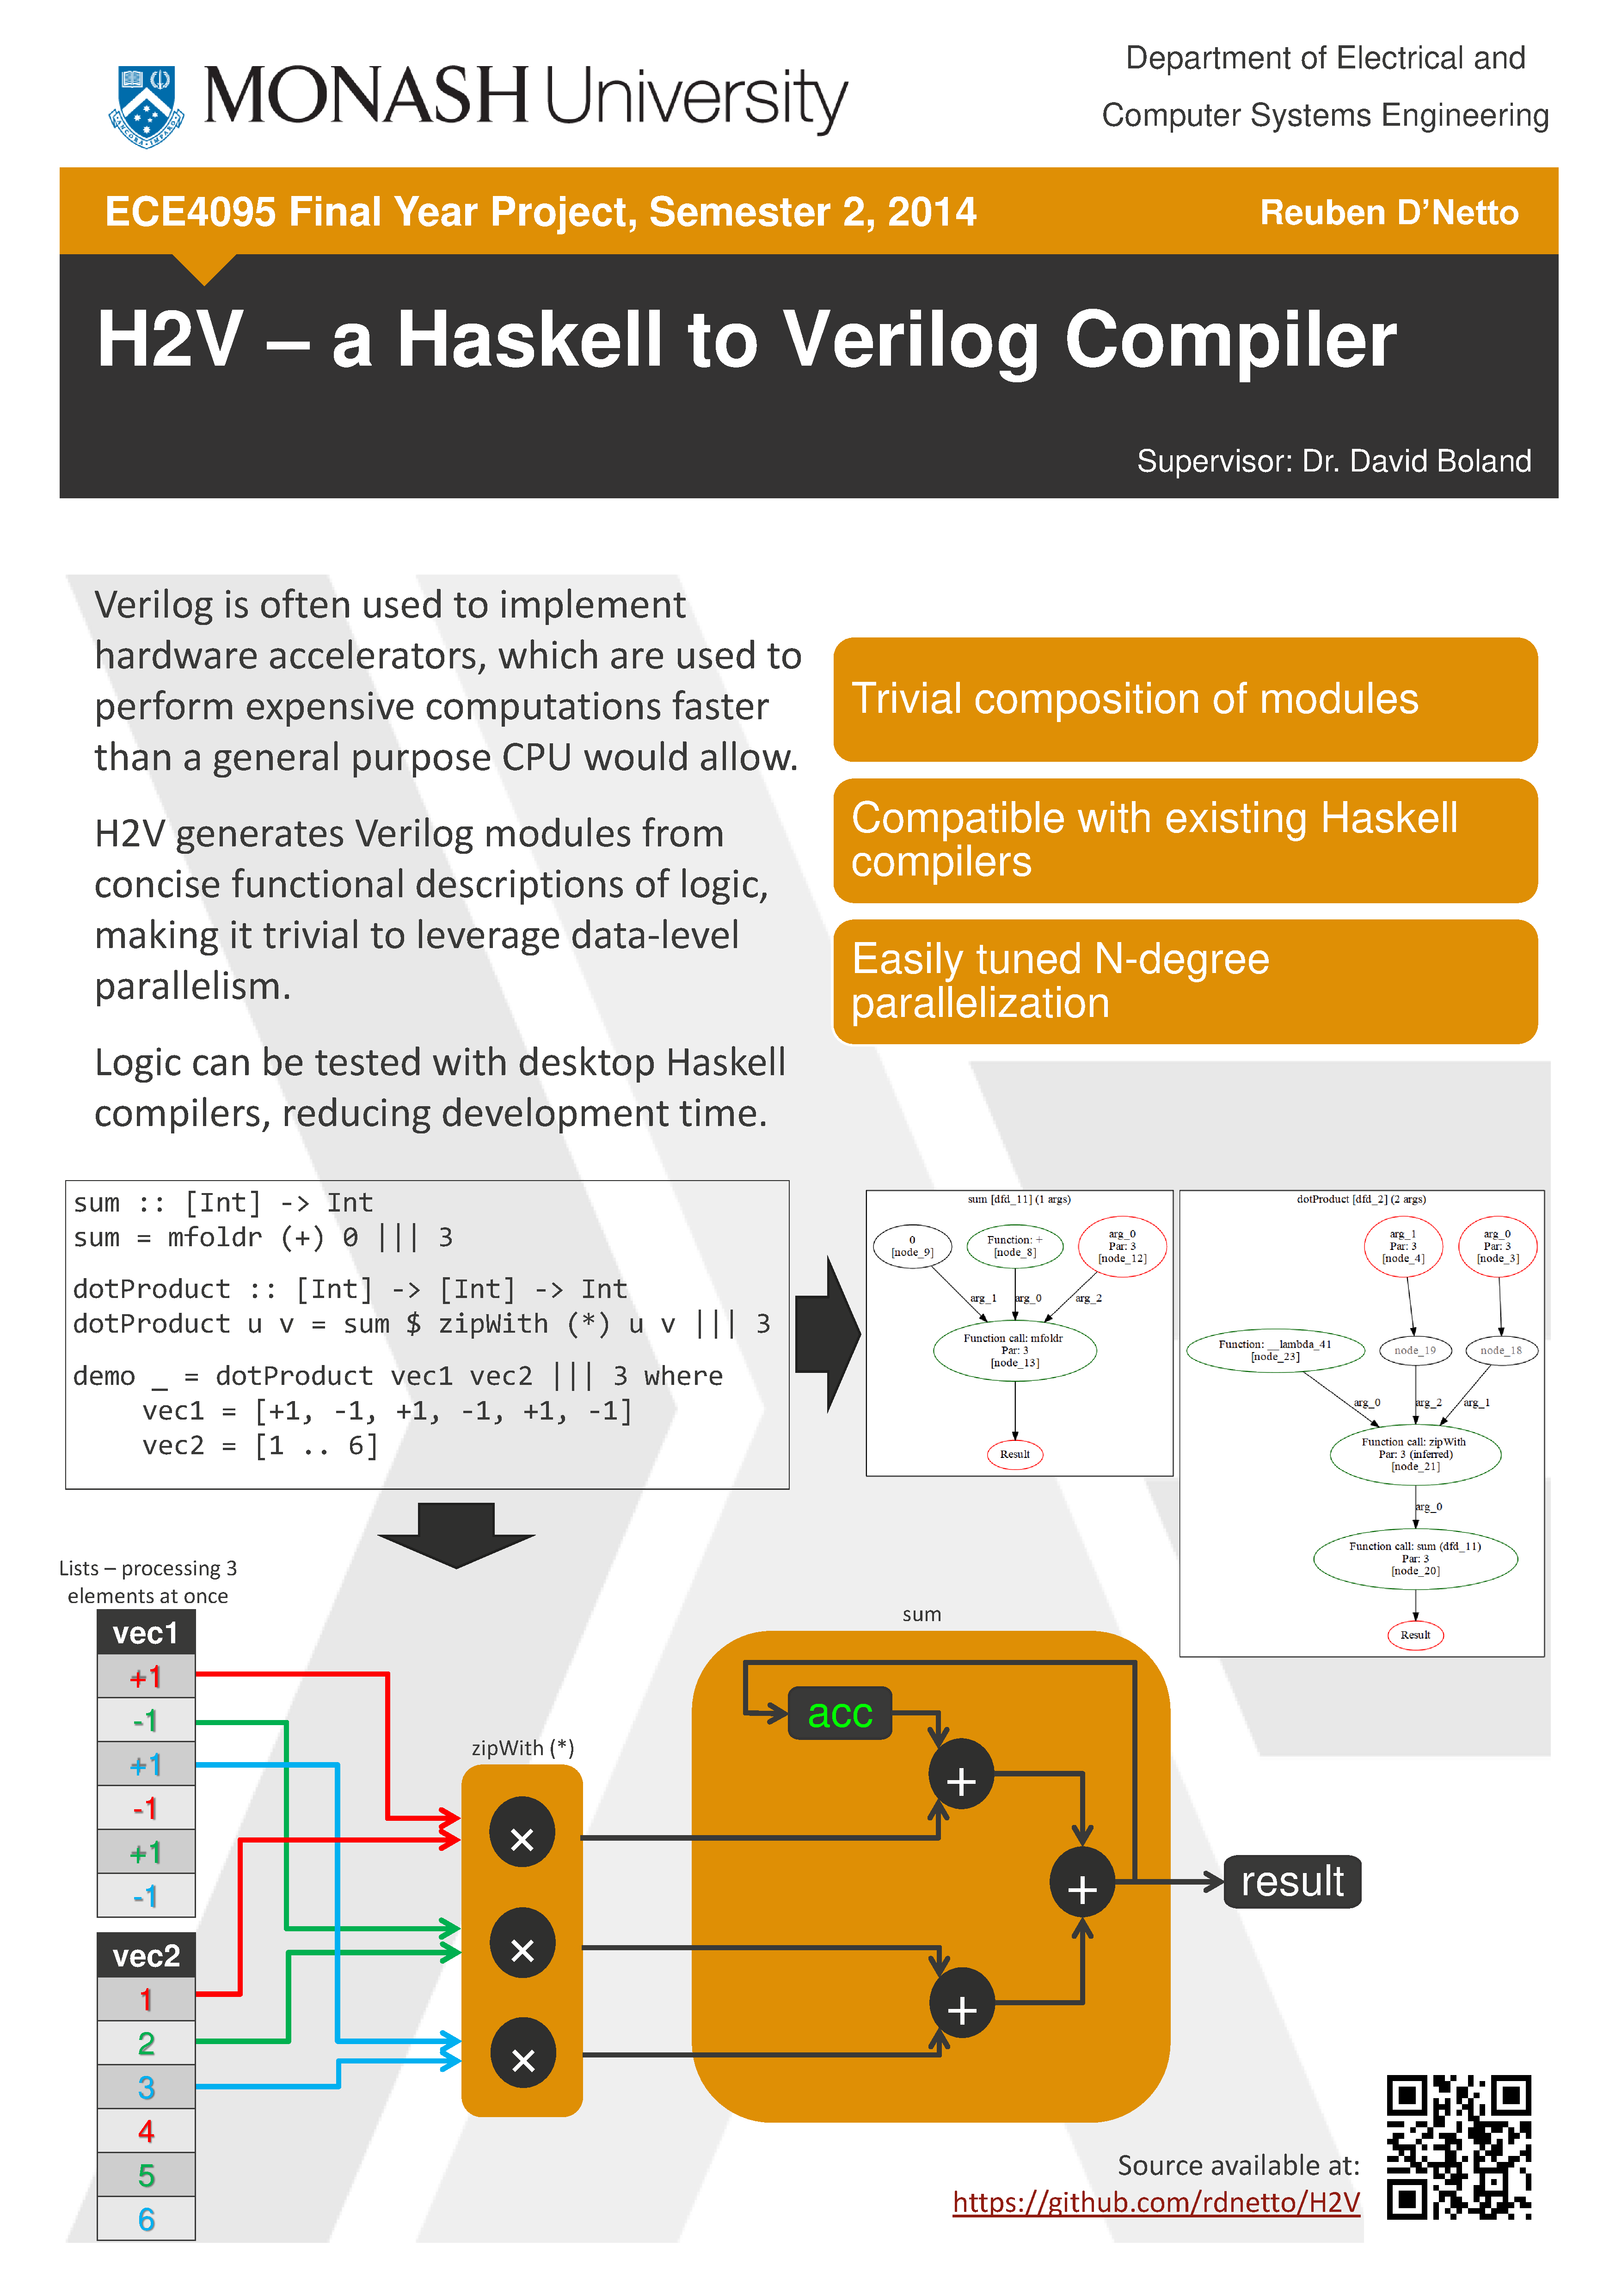
\includepdf[pages={1}, pagecommand={\invisiblesection{Poster}}]{../Poster/Poster.pdf}
\end{titlepage}

\section{Introduction}
\subsection{Context \& Rationale}
Verilog is a commonly used hardware description language used for programming field programmable gate arrays (FPGAs).
Its uses may be broadly grouped into two categories: interfacing with low-level hardware, and accelerating computations which
would otherwise be performed sequentially on a microprocessor. Due to its low-level nature (which is necessary for the first class
of use cases), implementing computations directly in Verilog is extremely time consuming, and often complex as a result of the
parallelism that it enables.

H2V is a Haskell to Verilog compiler. Programs can be defined extremely concisely and simply in Haskell, and then compiled into an
appropriate set of Verilog modules. Since H2V is compatible with a subset of the Haskell standard, the same program code can be
compiled and tested using existing tools, facilitating faster and more thorough testing.

\subsection{Haskell}
Haskell is a strongly typed pure functional language with lazy evaluation, in contrast to C, which is a weakly typed imperative
language with strict evaluation. This means that all variables in Haskell are immutable, and all functions are unable to access,
modify, or preserve any state. These features make it ideal for use in parallel computations, where state translates directly to
bottlenecks.%
\footnote{In fact, these features overlap considerably with the recommendations in many C to hardware tools.\cite{C2H_UG}}
Furthermore, because Haskell programs are defined in terms of the expressions assigned to variables (instead of the instructions
to be evaluated by a microprocessor), H2V has a much cleaner and more direct mapping between expressions and hardware modules than
C-based tools have.


\subsection{Project Definition}
The goal of this project is to demonstrate the viability of a Haskell to Verilog compiler, and its advantages over similar tools
which compile imperative programs (e.g.\ in C) to hardware. A Haskell to Verilog compiler (H2V) was implemented, but as a proof of
concept rather than a completed tool. H2V supports only a subset of the Haskell 2010 standard and the associated standard
libraries.


\section{Literature Review}

% Clash is a pain to type, so let's just define a command for it
\newcommand\Clash{C\(\lambda\)aSH}

\subsection{Academia}
The idea of using functional programming concepts to design hardware is not new; the concept dates back to the early
1980s,\cite[1135]{sheeran} prior to the standardization of Verilog\cite{Verilog_std} and VHDL.\cite{VHDL_std}
More modern attempts at doing so include Lava\cite{lava} and \Clash.\cite{clash}

Lava is an embedded domain-specific hardware description language, and as such intends each syntactic element to map to a hardware
block. This is achieved by encapsulating all signals in a abstract data type (called \texttt{Signal}), and breaks
compatibility with existing Haskell tools.
In contrast, H2V programs describe the computation of a value (or set of values), allowing the compiler more leeway for optimization.
For example, where a H2V program contains two multiplication operations as the children of a ternary operator (i.e.\ a multiplexor),
a single hardware multiplexor could be used without complicating the functional description.%
\footnote{This approach is already used in H2V for recursive functions, and could easily be applied to other cases such as
    expensive function calls.}

\Clash\ is more similar to H2V as it compiles a proper subset of Haskell to VHDL. It however lacks support for recursive
functions.\cite{clashReference}


\subsection{Commercial Tools}
There exists a large number of tools for compiling programs in C--like languages to hardware description languages,
such as Altera's C2H.\cite{C2H_UG} Many of them use proprietary extensions to compensate for the intrinsic deficiencies of
using a imperative system programming language for hardware, resulting in a highly fragmented landscape and the inability to use
existing C libraries.
In contrast to this, H2V programs are written in standard Haskell, and can use code from existing Haskell libraries (subject to
the limitations of its feature-set). Furthermore, using a functional language gives H2V some significant advantages over tools
based on imperative languages. (For a detailed discussion of this, please refer to s\ref{sec:imp_vs_func}.


\section{Supported Features}
\subsection{Comparison to Requirements Analysis}
\begin{tabularx}{\textwidth}{l c X c}
\toprule
ID      & Type              & Description                 & Implemented
\\ \midrule

3.1.1a  & Requirement & Support a subset of Haskell 2010. & Yes
\\ \midrule

3.1.1b  & Requirement & Support tail-recursive functions. & Yes
\\ \midrule

3.1.2.1 & Optional    & Retain compatibility with existing Haskell compilers. & Yes
\\ \midrule

3.1.2.2 & Optional    & Support first class functions. & Yes
\\ \midrule

3.1.2.3 & Optional    & Support unary non-tail recursive functions with bijective mappings for arguments. & No
\\ \midrule

3.1.2.4 & Optional    & Support for compiling multiple files at once. & No
\\ \midrule

3.1.2.5 & Optional    & Loop vectorization of recursive functions. & No
\\ \midrule

3.1.2.6 & Optional    & Restructuring of expression trees to reduce critical path. & No
\\ \midrule

3.1.2.7 & Optional    & Partial type inference. & Yes%
\footnote{Limited type inference is supported for scalar and list types. Type inference for higher-order types is not supported.}
\\ \midrule

3.2.1   & Requirement & QSys Integration --- generation of C headers and component definitions. & No%
\footnote{See s\ref{sec:reqQsys}.}
\\ \midrule

3.2.2.1 & Optional    & Use optional features in Avalon bus protocol to improve performance. & N/A
\\ \midrule

3.2.2.2 & Optional    & Support Avalon Streaming interfaces. & No
\\ \midrule

3.3.1   & Requirement & Support for sequential reads from RAM. & Implicit\footnotemark
\\ \midrule

3.3.2   & Optional    & Support for sequential writes to RAM. & Implicit\footnotemark[\value{footnote}]
\footnotetext{See s\ref{sec:reqDMA}.}
\\ \midrule

3.3.3   & Optional    & Support for non-sequential reads from RAM. & No
\\ \midrule

3.3.4   & Optional    & Support for caching subsequent accesses. & N/A
\\ \midrule

%TODO: it would be a really good idea to implement this for at least the demo case
3.4.1.1 & Requirement & Results shall include benchmarks comparing H2V and C2H. & No
\\ \midrule

3.4.1.2 & Requirement & The execution time of H2V accelerators shall be equal or better to those of C2H. & Yes%
\footnote{H2V is significantly faster than C2H in list-based benchmarks due to its support for parallelism
    (refer to s\ref{sec:listPar}.)}
\\ \midrule

3.5.1   & Requirement & H2V shall be published under a free software license. & Yes%
\footnote{H2V is available at \url{https://github.com/rdnetto/H2V} under the GNU General Public License version 2 (GPLv2).}
\\ \bottomrule
\end{tabularx}


\subsubsection{QSys Integration}
\label{sec:reqQsys}
QSys integration was abandoned as the goal of the project shifted from implementing a finished tool (a task that would likely take
years) to demonstrating the viability of the concept. QSys integration is trivial to implement, to the extent that it could easily
be performed by hand. Consequently, this would have added little to the project.

A second factor in abandoning QSys integration was that it relied on the inherent assumption that the main application of H2V was
augmenting Nios soft-processors. This proved to be false, as accessing data stored in the processor's RAM would be limited to two
words per cycle in most cases (due to the constraints of the hardware). In contrast, H2V achieves optimal performance in
applications where it can read several words in the same clock cycle. There would therefore be little point in implementing QSys
integration, as it would be advantageous only in situations where the Avalon bus was not memory-mapped.%
\footnote{The Avalon-MM bus has a maximum bandwidth of 128 bytes per clock cycle,\cite[3-4]{C2H_AvalonSpec} and so could be connected
    to H2V modules without a significant reduction in throughput.}


\subsubsection{Direct Memory Access}
\label{sec:reqDMA}
Instead of implementing direct memory access, a well-defined list interface protocol was implemented. This has the advantage of
enabling parallelism beyond what the memory would support, as well as offering increased flexibility in allowing a variety of data
sources and sinks to be used. Since all related use cases in the requirements analysis have been satisfied, this requirement can
be regarded as completed.


\subsection{Supported Features}
% discuss exactly what is supported here, possibly in terms of test suite

\subsubsection{Language Features}
H2V is capable of correctly resolving functions and variables defined out of order in multiple scopes, including shadowing.\ i.e.\ the
definition in the innermost scope has precedence over definitions in outer scopes with the same name. Pattern guards and pattern
matching are also supported; the function definitions are lowered into a single definition with appropriate if statements /
multiplexors inserted at the root node. Tail-recursive functions are supported, with pattern matching is used to define the base and
recursive cases.

Refer to s\ref{sec:testLangFeat} for test cases corresponding to these features.


\subsubsection{Higher-Order Functions}
\paragraph{Introduction}
The following section is for the benefit of readers who are unfamiliar with the concept of higher-order functions, and may be
skipped.

Consider a function of the form \(f:(x, y) \rightarrow z | f(x, y) = x + y\). This is a function of arity 2 (i.e. it takes two arguments) and
order one; it is a first-order function. In general, any function whose argument and return types are scalar types (or lists
thereof) is a first-order function. Variables, which do not take any arguments, may be regarded as zeroth-order functions.
In other words, first-order functions take arguments and return values which are zeroth-order functions.

This may then be generalized in a manner similar to induction, to define an Nth-order function as one which takes arguments and
returns a value of order \(N - 1\) or lower.\footnotemark Functions of order two or higher are generally referred to as
higher-order functions, in contrast to first-order functions.
\footnotetext{Any function can trivially be expressed as one of a higher order, by defining a function which returns the original
    function.}

In Haskell, all functions of arity two or higher are considered higher-order functions, since partial application (i.e. the
application of fewer arguments than the arity of the function) of a function returns a function which takes the remaining
arguments.\footnote{This is referred to as \textit{currying}, after the logician Haskell Curry.}
While H2V supports partial application, the following discussion will refer to first-order functions of any arity as first-order
functions, in order to simplify the terminology.

It is worth taking the time to distinguish higher-order functions in Haskell from function pointers in C. Function pointers allow
functions to take arguments and return values which are pointers to existing functions. This is more limited than higher-order
functions, which allow completely new functions to be returned.%
\footnote{While one could theoretically allocate some memory, write assembly to it, and return a pointer to it in C, the
    resulting code would not be portable, and would certainly not be usable in C2H. A more sensible approach would be provide a
    pointer to a data structure, but this would be shared state which would prevent the function being called multiple times in
    parallel.}
Furthermore, the function pointer cannot be modified in anyway, while higher-order functions in Haskell can have arguments applied
to them, to yield new functions via partial application. This is a direct consequence of the languages' different philosophies:
Haskell was designed to represent computations, while C was designed to represent machine code, in which a function is merely a
memory address to be jumped to.


\paragraph{Implementation}
Because a functional argument may be evaluated multiple times within a higher-order function, it is impractical to pass it at
run-time. Therefore, H2V implements support for higher-order functions by evaluating them at compile-time, effectively rewriting
them as first-order functions which are evaluated at run-time. This is sufficient as higher-order functions are used primarily to
enable code re-use rather perform expensive computations. For example, Haskell's map function (see s\ref{sec:listFuncs}) is a
higher-order function which maps a list over its functional argument. The partial application \texttt{map f} yields a first-order
function which performs that same mapping. The application of the functional argument is a relatively cheap operation that can be
performed at compile-time (simply substituting the function into the data flow graph), while the evaluation of the resulting
first-order function is an expensive operation depending on the contents of the list at run-time.

Examples of higher-order functions supported by H2V may be found in s\ref{sec:testHOFunc}.

\subsubsection{Lists}
\paragraph{Concept}
Lists in H2V are implemented as a streaming data source. This is mirrors Haskell's lazy evaluation, where values (such as the
elements of the list) are not computed until they are required. This means that lists can be used to encapsulate data without
adding significant overheads, in contrast to C where arrays are mapped to blocks of memory. Furthermore, it means that the total
memory requirements of the data structure are restricted to the number of elements accessed at any one time. This means that lists
can be of infinite length.\ e.g.\ \texttt{[1, 3 ..]} will evaluate to the list of all positive odd numbers.

\paragraph{Parallelism}
\label{sec:listPar}
List operations are a prime candidate for parallelism, since the data is already organized into discrete elements which are
subject to the same repeated operations. To facilitate this, H2V defines a parallelism operator \texttt{|||} which may be applied
to any expression which returns a list to define the number of elements it should read/process simultaneously. Parallelism
inference is supported within functions; that is, any parallelism assignment will be propagated to other adjacent nodes in the
data flow graph.

\paragraph{Higher-order List Functions}
\label{sec:listFuncs}
H2V supports three higher-order list functions: \texttt{map}, \texttt{mfoldr}, and \texttt{zipWith}.
\texttt{map} applies a function to each element of a list, returning a list containing the result of each application.
\texttt{zipWith} generalizes map to functions with two arguments, taking the first and second arguments from their respective
lists. Both of these functions request values from the source list and start computing the result before the consumer of the
resulting list attempts to read from it, ensuring that all reads after the first take only one clock cycle (provided that the
computation has had enough time to complete).

\texttt{mfoldr} is a monoidic right-fold. Fold (or reduce as it is sometimes known) recursively applies a function to an element
of the list and an accumulator, storing its value in the accumulator. Right and left folds refer to the order in which the
elements of the list are processed. Because the order in which elements are folded is defined for \texttt{foldr} and
\texttt{foldl}, it is not possible to compute folds in parallel. For this reason the function \texttt{mfoldr} was defined instead.
\texttt{mfoldr} imposes the additional constraint that the function and its domain form a \textit{monoid}.%
\footnote{A monoid is an algebraic structure consisting of a set and a binary function which is associative and has a
    right-identity over the that set. For example, addition is a monoid over the set of real numbers with a right-identity of 0.}
By adding the requirement that the function must be associative, intermediate values can be computed in parallel using a binary
reduce tree. The use of a right-identity instead of an initial value for the accumulator also means that the number of values read
from the list can be an arbitrary number instead of a power of two, since the empty slots can simply be set to the identity,
thereby having no effect on the result.

%TODO: insert diagrams to explain list functions


\subsection{Case Study --- Dot Product}
\label{sec:imp_vs_func}
Consider the following C code for computing a Euclidean inner product. (i.e.\ a vector dot product)
The \texttt{\_\_restrict\_\_} type qualifier allows the compiler to assume pointer aliasing does not occur,\cite[122]{c_std}
and a hypothetical pragma is used to instruct the compiler to unroll three iterations of the loop.

\begin{lstlisting}[language=C]
    int dotProduct(const int* __restrict__ listA, const int* __restrict__ listB, int length){
        int result = 0;

        #pragma unroll_loop_with_parallelism 3
        for(int i = 0; i < length; i++)
            result += listA[i] * listB[i];

        return result;
    }
\end{lstlisting}

If we consider how it maps to hardware, the following questions arise:
\begin{itemize}
    \item How is the summation performed? Does each sum occur after \texttt{result} is updated, or is there an intermediate
            reduction tree?
    \item Does the pragma indicate that three elements should be read from each list, or that three operations should be
        performed? Are either of these interpretations even logically possible, and if not, will the compiler issue an error?
    \item How many values are read from \texttt{listA} and \texttt{listB} each cycle?
    \item Does the hardware attempt to sum and multiply the same number of values per clock cycle, or is it aware that these
            operations take different durations to complete?
    \item Is it possible for the values in \texttt{listA} and \texttt{listB} to be modified during the computation? C's
        \texttt{const} keyword only protects access to a location in memory via a given variable, not the memory location itself.
        \ i.e.\ the elements of the list are not \textit{immutable.}
\end{itemize}

It quickly becomes obvious that even with an explicit pragma for controlling loop unrolling, there is a lot of ambiguity as to how
the compiler generates the hardware. This is partly due to the conflation of two different operations: the addition and
multiplication. Because they are combined into construct in idiomatic C, it becomes difficult to analyze them in isolation, even
though they are separate operations computationally and would ideally map to separate blocks of hardware. The following code
addresses this problem.

\begin{lstlisting}[language=C]
    int dotProduct(const int* __restrict__ listA, const int* __restrict__ listB, int length){
        int result = 0;
        int tmp[length];

        #pragma unroll_loop_with_parallelism 3
        for(int i = 0; i < length; i++)
            tmp[i] = listA[i] * listB[i];

        #pragma unroll_loop_with_parallelism 3
        for(int i = 0; i < length; i++)
            result += tmp[i];

        return result;
    }
\end{lstlisting}

This allows us to define the parallelism of the addition and multiplication separately, but the other problems remain.
Furthermore, we now have to consider how the compiler treats \texttt{tmp[]}:
\begin{itemize}
    \item Is a block of memory allocated for \texttt{tmp}, or does the compiler recognize it is used as an intermediate variable?
            Can the compiler identify that its elements are consumed in order, or does it store the contents to allow for
            random-access?
    \item How does the compiler handle cases where the loops have different parallelisms? Will it warn the programmer, or simply
            assume it was intended? This is significant, as the connection between data sources and sinks may be completely
            unobvious in a large program.
\end{itemize}
Perhaps most importantly, the code is no longer idiomatic, and can hardly be considered elegant. Elegance and idiomacy are
important because they indicate syntactic and computational structures which are easily understood and recognized by both humans
and computers, and are therefore easily optimized by compilers.

Finally, consider the following function, which generalizes the previous definition by replacing the operators with arbitrary
functions.

\begin{lstlisting}[language=C]
    int innerProd(const int* __restrict__ listA, const int* __restrict__ listB, int length){
        int result = 0;
        int tmp[length];

        #pragma unroll_loop_with_parallelism 3
        for(int i = 0; i < length; i++)
            tmp[i] = func1(listA[i], listB[i]);

        #pragma unroll_loop_with_parallelism 3
        for(int i = 0; i < length; i++)
            result = func2(result, tmp[i]);

        return result;
    }
\end{lstlisting}

In addition to the previous concerns, the programmer must now consider whether \texttt{func1} and \texttt{func2} are
\textit{pure}. A pure function is one whose evaluation does not depend on any shared state. Such state restricts parallelism,
creating bottlenecks and race conditions. In a small program it may be reasonable for the programmer to keep track of such things
mentally, but this cannot be said of larger programs authored by entire teams, and any solution which assumes humans will not make
mistakes is no solution at all.

Now let's consider the idiomatic solution to the same problem in Haskell.

\begin{lstlisting}
    sum :: [Int] -> Int
    sum = mfoldr (+) 0 ||| 3

    dotProduct :: [Int] -> [Int] -> Int
    dotProduct listA listB = sum $ zipWith (*) listA listB ||| 3
\end{lstlisting}

We have defined \texttt{sum} as a separate function for clarity, but it is immaterial whether it is manually inlined or not.
Given this code, we can now easily answer the questions from before.
\begin{itemize}
    \item Summation (\texttt{mfoldr (+)}) and multiplication (\texttt{zipWith (*)}) are clearly distinct operations,
        and can be annotated using the parallelism operator (\texttt{|||}) to indicate how many elements should be read at a time.
        Because this is an operator and not a pragma, it can be used multiple times per line on different expressions.
        An additional benefit of clearly separating these operations is that it simplifies resource sharing.
        (see s\ref{sec:resSharing}.)
    \item Summation is performed using \texttt{mfoldr}, which uses a reduction tree by definition.
    \item As Haskell is a functional language, all variables are guaranteed to be immutable and all functions to be pure,
        so the compiler is able to optimize the function as aggressively as possible without needing to perform expensive,
        link-time analysis to verify this.
    \item Since Haskell uses lazy evaluation, the output of \texttt{zipWith} is not even computed until it is needed by
        \texttt{sum}. This means that there is no overhead, and both operations can be performed in parallel on the data stream.
    \item If \texttt{sum} has a different parallelism to \texttt{dotProduct}, H2V will give the user an error message.
\end{itemize}

Furthermore, the code is idiomatic and concise. It is identical to the equivalent code in standard Haskell (minus the parallelism
annotations), and a mere four lines long (reducible to two if \texttt{sum} is inlined), in contrast to the eleven lines of C.
Put simply, the Haskell version maps as cleanly to hardware as C does to assembly, as shown in Figure~\ref{fig:dotProdBD}.

\begin{figure}[h]
\includegraphics[keepaspectratio=true,width=\textwidth]{"Dot Product Block Diagram".pdf}
\caption{Hardware generated by H2V for dot product definition.}
\label{fig:dotProdBD}
\end{figure}
\pagebreak{}

\subsection{Interfaces \& Protocols}
\subsubsection{Function Interface}
\label{sec:funcInterface}
All functions compiled into Verilog modules by H2V use the following interface.

\begin{tabularx}{\textwidth}{l l l X}
\toprule
Name        & Width     & Type      & Description
\\ \midrule

\texttt{clock}         & 1 bit     & Input     & Clock signal.
\\ \midrule

\texttt{ready}       & 1 bit     & Input     & Clock enable --- indicates that the other input values are now valid.
\\ \midrule

\texttt{done}        & 1 bit     & Output    & Asserted high when \texttt{result} is valid.
\\ \midrule

\texttt{arg0, arg1, \ldots}  & 8 bits\footnotemark & Input    & The values passed to the function as arguments.
\\ \midrule

\texttt{result} & 8 bits\footnotemark[\value{footnote}] & Output    & The return value of the function.
\\ \bottomrule
\end{tabularx}
\footnotetext{8 bits is the default width for scalar values --- see s\ref{sec:parListComp}. Refer to s\ref{sec:listInterface} if the argument is a list.}

\begin{figure}[h]
\begin{tikztimingtable}[scale=2, line width=1]
    clock  &  9{C}       \\
    ready  &  L 6H 2L    \\
    args   &  U 6D 2U    \\
    done   &  U 2L 4H 2U \\
    result & 3U 4D 2U    \\
\end{tikztimingtable}
\caption{Timing diagram for function interface.}
\label{fig:funcTiming}
\end{figure}

\subsubsection{List Interface}
\label{sec:listInterface}

Arguments which are lists are passed using the following signals:

\begin{tabularx}{\textwidth}{l l l X}
\toprule
Name        & Width     & Type      & Description
\\ \midrule

\texttt{REQ}       & 1 bit     & Input      & Asserted high when a new (set of) elements are requested. One asserted, must be
    reset before another request can be made. Note that \texttt{value\_0, \ldots} will only remain valid as long as \texttt{REQ} is
    high.
\\ \midrule

\texttt{ACK}        & 1 bit     & Output    & Asserted high for one clock cycle when \texttt{value\_0, \ldots} become valid.
\\ \midrule

\texttt{value\_0, \ldots}  & 8 bits & Output    & The values of the next N elements, where N is the parallelism of the list
instance.
\\ \midrule

\texttt{value\_0\_valid, \ldots}  & 1 bit & Output    & Asserted high if \texttt{value\_0, \ldots} are valid.
\\ \bottomrule
\end{tabularx}

\begin{figure}[h]
\begin{tikztimingtable}[scale=1.5, line width=1]
    clock & 25{C} \\
    req             &  L 3{6H2L}   \\
    ack             &  L 3{2L2H4L} \\
    value\_0        & 3U 4D{$X_0$} 4U 4D{$X_3$} 10U \\
    value\_1        & 3U 4D{$X_1$} 4U 4D{$X_4$} 10U \\
    value\_2        & 3U 4D{$X_2$} 4U 14U  \\
    value\_0\_valid & 3U 4H 4U 4H 4U 4L 2U \\
    value\_1\_valid & 3U 4H 4U 4H 4U 4L 2U \\
    value\_2\_valid & 3U 4H 4U 4L 4U 4L 2U \\
\end{tikztimingtable}
\caption{Timing diagram for the list interface of \(\{X_0, X_1, X_2, X_3, X_4\}\).}
\label{fig:listTiming}
\end{figure}

Note that each list has an integral parallelism.\ i.e.\ the number of values read per \texttt{REQ--ACK} cycle.
It is an invariant of the interface that
\[ \texttt{value\_i\_valid} \implies \texttt{value\_j\_valid}\ \forall\ i > j \]

If \texttt{value\_0\_valid} is asserted low, then the end of the list has been reached. Note that as H2V supports infinite lists,
there is no guarantee that this signal will ever be asserted low.

The signals \texttt{value\_i} and \texttt{value\_i\_valid} are only valid
for the interval between \texttt{ACK} being asserted and \texttt{REQ} being unasserted.


\pagebreak{}
\section{Future Work}
As stated previously, H2V is a proof of concept; it provides a foundation for a complete tool to be built upon.
The following sections describe features that would be needed to realize this vision, and discuss the extent to which the existing
codebase supports them.

\subsection{Improved Type Support}
\subsubsection{Variable Width Integers}
H2V currently supports only two scalar types: booleans and unsigned 8-bit integers. To be useful in real applications,
support for signed integers and integers of other sizes will be needed. H2V's type system already supports these,%
\footnote{See \texttt{DType} at \texttt{H2V/DfdDef.hs:100} for a complete description of H2V's type system.}
so implementing support is a simple matter of extending the parsing and rendering logic.
Bit-widths could be described using parameterised types. For example, a signed 16-bit integer would be expressed as
\texttt{SInt 16}. An advantage of using parameterised types is that the user can specify any width, rather than just
one of a predefined set. This can result in significant reductions in hardware used for expensive computations, such as
multiplication. Aliases could also be defined for \texttt{Word8}, \texttt{Word16}, etc.\ as unsigned integers and \texttt{Int8},
\texttt{Int16}, etc.\ as signed integers to preserve compatibility with existing Haskell code.

\subsubsection{Fixed-point Types}
Similarly, fixed-point types could also be defined.\ e.g.\ \texttt{FP 4 8} would describe a fixed-point number with 4 integer bits
and 8 fractional bits. An advantage of this over existing approaches in C is that the compiler would be able to combine types
correctly. Consider the following Haskell, and the equivalent C.

\begin{lstlisting}[language=C]
    int add1_to_fp8(int x){
        return x + (1 << 8);
    }
\end{lstlisting}

\begin{lstlisting}
    add1 :: FP 4 8 -> FP 4 8
    add1 x = x + 1
\end{lstlisting}

In the C example, a bit-shift is needed to convert 1 from an integer to a fixed-point type, which obscures the actual function of
the code. This is completely unnecessary in the Haskell example, because the compiler can recognize the need for type conversion
and perform it automatically. Given that bit-shifts are effectively free when performed in hardware, there is no reason for the
programmer concern themselves with this detail, and the bit-shift present in the C obscures the true purpose of the code. While
this may seem insignificant for such a trivial example, reading such code becomes considerably more difficult when evaluating
complex expressions.


\subsubsection{Nested Lists}
A significant limitation of H2V is that it is currently only able to manipulate one-dimensional lists. This is particularly
limiting since H2V's streaming approach to list manipulation means it is impossible to index an element of the list without
discarding everything prior to it. Nested lists would allow representation of multi-dimensional data, such as images.
For instance, matrices could also be intuitively represented as a list of rows with a type such as \texttt{[[Int]]}.

H2V's type system already supports nested lists, since it defines lists recursively (i.e.\ a list is a type parameterised in any
other type, including itself). As the function interface\footnote{See s\ref{sec:funcInterface}.} currently states that lists are
handled by replacing the single scalar port for those described by the list interface,\footnote{See s\ref{sec:listInterface}.}
it would be logical to do the same for the list interface.\ i.e.\ instead of requiring \texttt{list\_value\_0} to be a scalar, it
could be replaced by the full set of ports defined by the list interface. This would also be particularly easy to implement, since
functions for rendering nodes as either scalars or lists (depending on type) with a prefix already exist.%
\footnote{E.g. \texttt{renderArg} at \texttt{H2V/RenderVerilog.hs:340}.}

One complexity that arises from this is the semantics of the parallelism operator when used with nested lists, and whether it
applies to all levels of the list or just the outermost. In order to be consistent, it should apply to the outermost level only,
so that the element type (i.e.\ the inner lists) are treated the same regardless of whether they are scalar or not.
In order to describe the parallelism of nested lists, it becomes desirable to define a new operator. This could be called the
multi-dimensional parallelism operator, and would take a list of integers instead of a single one, with each element of the list
assigning a parallelism to the lists of corresponding depth.\ e.g.\ \texttt{[[1, 2], [3, 4], [5, 6]] ||* [3, 2]} would assign a
parallelism of 3 to the outer list and 2 to the inner list, while \texttt{[[1, 2], [3, 4], [5, 6]] ||| 3} would only assign a
parallelism to the outer list.


\subsection{Type \& Parallelism Inference}
H2V currently supports type and parallelism inference within functions. However, each function must have its own type signature
and parallelism assignment. This quickly becomes unwieldy, as demonstrated by \texttt{demo.hs} on page~\pageref{test:demo}. Allowing
parallelism to be inferred across function boundaries would render the redundant assignments unnecessary and improve code re-use
by allowing the same function to be called in different places with different parallelisms.

Type inference would facilitate code re-use by enabling generic functions. For example, consider the following second-order functions:

\begin{lstlisting}
    applyTwice1 :: (Int -> Int) -> (Int -> Int)
    applyTwice1 f = \x -> f (f x)

    applyTwice2 :: (a -> a) -> (a -> a)
    applyTwice2 f = \x -> f (f x)
\end{lstlisting}

The first instance can only be used for functions of \texttt{Int}s, while the second can be used for any function whose argument
and return value are of the same type. In order for the same function to be called with differently typed arguments in different
places, the compiler would need to track the types it was called with, which is the same information that would be needed for type
inference.


\subsection{Closures}
Closures extend first-order functions by allowing them to reference variables in their defining context.\ i.e.\ they are said to
\textit{close over} said variables. Consider Listing~\ref{lst:closure}, which defines a function that increments every element of
a list by the provided value. The inner function \texttt{f} closes over the variable \texttt{a}, which is a member of
\texttt{incrementAll}. As Verilog does not allow for nested modules, the function must be rewritten by the compiler so that the
only inputs take the form of module parameters.

H2V currently has experimental, untested support for closures.%
\footnote{See \texttt{H2V/GenerateDFD.hs:730}.}
As part of the linking process, it identifies each function which contains references variables defined outside it,
adds them to its list of arguments, then updates all of the calls to that function to include the closed over variables.

\begin{figure}
\begin{lstlisting}
    incrementAll :: Int -> [Int] -> [Int]
    incrementAll a xs = map f xs where
        f x = x + a
\end{lstlisting}
\caption{A function with a closure.\label{lst:closure}}
\end{figure}


\subsection{Compilation of Recursive List Functions}
\label{sec:parListComp}
H2V currently implements \texttt{map}, \texttt{zipWith} and \texttt{mfoldr} using hard-coded functions for generating their logic.
This approach scales extremely poorly, requiring approximately 150 lines of dedicated code for each one,%
\footnote{See \texttt{H2V/RenderVerilog.hs:669}.}
and means imposes a significant implementation cost for each such function. Ideally, these functions could be defined in Haskell
(as shown in Listing~\ref{lst:recListFuncs}), and generalized logic used to compile them.
This would enable the re-use of existing list functions from the standard library, significantly boosting the expressive power of H2V.

\begin{figure}
\begin{lstlisting}
    map :: (a -> b) -> [a] -> [b]
    map f (x0:xs) = (f x0) : (map f xs)

    zipWith :: (a -> b -> c) -> [a] -> [b] -> [c]
    zipWith f (x0:xs) (y0:ys) = (f x0 y0) : (zipWith f xs ys)

    foldl :: (b -> a -> b) -> b -> [a] -> b
    foldl f z (x0:xs) = foldl f (f z x0) xs
    foldl f z [] = z

    foldr :: (a -> b -> b) -> b -> [a] -> b
    foldr f z (x0:xs) = f x0 (foldr f z xs)
    foldr f z [] = z

    sumEachPair :: [Int] -> [Int]
    sumEachPair (x0:x1:xs) = (x0 + x1) : (sumEachPair xs)
\end{lstlisting}
\caption{Haskell definitions of recursive list functions.\label{lst:recListFuncs}}
\end{figure}

This feature could be implemented by recognizing that all of these cases involve recursive functions which consume or produce
lists, in both cases via the cons operator (\texttt{:}). We can then extract the expressions for the elements to be prepended to
the list, and compile them to the appropriate logic, connected to a list interface. Loop unrolling can be applied as usual via the
parallelism operator. Note that specialized logic would still be required for the monoidic fold functions (e.g. \texttt{mfoldr}),
as their implementation relies on the non-syntactic constraint that the folding function and its domain are a monoid.%
\footnote{See s\ref{sec:listFuncs}.}

An attempt was made at implementing this, but was not completed due to time constraints. It can be found on the topic branch
\texttt{recursive\_list\_functions}.


\subsection{Resource Sharing}
\label{sec:resSharing}
In complex programs, it is rare for all hardware blocks to be in use simultaneously. Because functional programming encourages
the expression of programs as many small, modular functions, it becomes viable to identify commonly used functions and re-use
existing hardware blocks when the calls are known to happen at mutually exclusive times. For example, consider the example
code in s\ref{sec:imp_vs_func}. Identifying the re-usable code in the C example would be extremely difficult; at most one could
make some arguments about individual multipliers. However, the Haskell code clearly groups the operations using
\texttt{mfoldr (+)} and \texttt{zipWith (*)}, and even explicitly assigns them parallelisms.
Generalizing further, the \texttt{dotProduct} function as a whole could be re-used in multiple places.
This would require a significant amount of effort as H2V currently does not consider timing requirements or
the relationships between different modules, but could result in some fairly impressive reductions in hardware requirements,
especially for applications like CPUs where only a small fraction of the ALU is in use at any given time.


\section{Conclusions}
The results of this project demonstrate the feasibility of generating hardware descriptions from functional programs.
Language features are easily rewritten to equivalent Verilog constructs and higher-order functions can be effectively
evaluated at compile-time. The streaming model for lists was found to work extremely well, though the lack of support for nested
lists and recursive functions of lists prevented its application to problems involving matrices. Extending the range of supported
types, improving inference and adding features such as closures and native compilation for recursive functions are recommended,
as this will result in the creation of an extremely powerful and elegant hardware synthesis tool.

\pagebreak{}
\appendix
\section{Appendix --- Test Cases}
The following test suite is representative of the kinds of programs H2V is capable of compiling. Each test case is followed by the
DFD generated by H2V. Verilog output has been omitted for brevity.

The test suite can be run on a UNIX-compatible system using the following commands:

\begin{lstlisting}[language=bash]
    git checkout https://github.com/rdnetto/H2V.git
    cd H2V/tests
    ./test-all.sh
\end{lstlisting}

% Define a command to avoid repetition and handle underscores correctly
% Based on: http://tex.stackexchange.com/questions/38536/how-can-i-pass-underscore-to-newcommand-properly
\newcommand\insertTestCase{\begingroup\catcode`_=12 \doInsTC}
\newcommand\doInsTC[2]{
    \minipage{\linewidth}
        \label{test:#1}
        \lstinputlisting{../../H2V/tests/#1.hs}
    \endminipage
    \begin{figure}[htbp]
        \includegraphics[keepaspectratio=true,#2]{../../H2V/tests/#1}
        \caption{DFD for \texttt{#1.hs}}
    \end{figure}}

\subsection{Language Features}
\label{sec:testLangFeat}
\insertTestCase{f0}{scale=0.25}
\insertTestCase{f1}{scale=0.25}
\insertTestCase{guards}{scale=0.25}
\insertTestCase{pattern_match}{width=\textwidth}
\insertTestCase{fib}{width=\textwidth}

\subsection{Higher-Order Functions}
\label{sec:testHOFunc}
\insertTestCase{ho_arg}{width=\textwidth}
\insertTestCase{ho_flip}{width=\textwidth}
\insertTestCase{ho_pa}{width=\textwidth}
\insertTestCase{ho_return}{width=\textwidth}

\subsection{Lists}
\label{sec:testList}
\insertTestCase{lists}{width=\textwidth}
\insertTestCase{lists2}{width=\textwidth}
\insertTestCase{demo}{width=\textwidth}

\section{Appendix --- Source Code}
The source code is available at \url{https://github.com/rdnetto/H2V}.

\section{Appendix --- Include Files for H2V Programs}
The following files should be included by H2V programs. \texttt{H2V\_Compat} enables existing Haskell compilers to work with H2V
code by defining non-standard functions and operators. \texttt{include.v} contains Verilog modules used by generated code and must
be added to any Quartus project using H2V modules.

\lstinputlisting{../../H2V/include/hs/H2V_Compat.hs}
\lstinputlisting{../../H2V/include/v/include.v}

\pagebreak{}
\printbibliography
\end{document}

